\documentclass{article}
\usepackage[utf8]{inputenc}
\usepackage[spanish]{babel}
\usepackage{graphicx}
\usepackage{geometry}
\usepackage{enumerate}
\usepackage{titlesec}
\usepackage{float}
\usepackage{listings}
\usepackage{xcolor}
\usepackage{amsmath}
\usepackage{matlab-prettifier}
\usepackage{amssymb}
\usepackage{tabularx}

\geometry{letterpaper, margin = 1.5cm}

\newcommand{\codefontsize}{\fontsize{10}{11}}
\lstset{
	style = Matlab-editor,
	basicstyle = \codefontsize\ttfamily,
	mlshowsectionrules = true,
	upquote = true,
	tabsize = 4,
	captionpos = b,
	breaklines = true,
	breakatwhitespace = true,
	frame = single,
}

%Datos de la Portada
\title{Introducción a la Programación \ Practica 10}
\author{Medina Martinez Jonathan Jason \ 2023640061}
\date{11 de junio del 2023}

\begin{document}
	
	\fontsize{12}{16}\selectfont
	
	\begin{figure}[t]
		
		
\includegraphics[width=2.5 cm]{Logo1.jpeg}
		\hfill
		
\includegraphics[width=3 cm]{Logo2.png}
		
	\end{figure}
	
	\maketitle
	\newpage
	
	\tableofcontents
	\newpage
	
	\section{Objetivo}
	
	Desarrollo de un bloque de trabajo utilizando el ambiente grafico de simulación.
	
	\section{Introducción}
	
	En el campo de la simulación y procesamiento de imágenes, el uso de ambientes gráficos de simulación se ha vuelto fundamental para desarrollar soluciones efectivas. En esta práctica, nos enfocaremos en el uso de Simulink, una herramienta ampliamente utilizada, para crear un bloque de trabajo que permita adquirir video desde una cámara web, aplicar una serie de transformaciones a la imagen y visualizar el video resultante. El objetivo es familiarizarse con el entorno gráfico de Simulink y explorar cómo se pueden utilizar sus capacidades para el procesamiento de imágenes en tiempo real.
	
	\newpage
	
	\section{Desarrollo}
	
	Utilizando Simulink, cree un diagrama de bloques que permita:
	
	\begin{itemize}
		\item Adquirir video desde la cámara web.
		\item Convertir la imagen a escala de grises.
		\item Aplicar un filtro Sobel a la imagen en escala de grises.
		\item Invertir la imagen resultante.
		\item Mostrar el video resultante en pantalla.
	\end{itemize}
	
	\newpage
	
	\subsubsection{Modelo}
	
	\begin{figure*}[h]
		\centering
		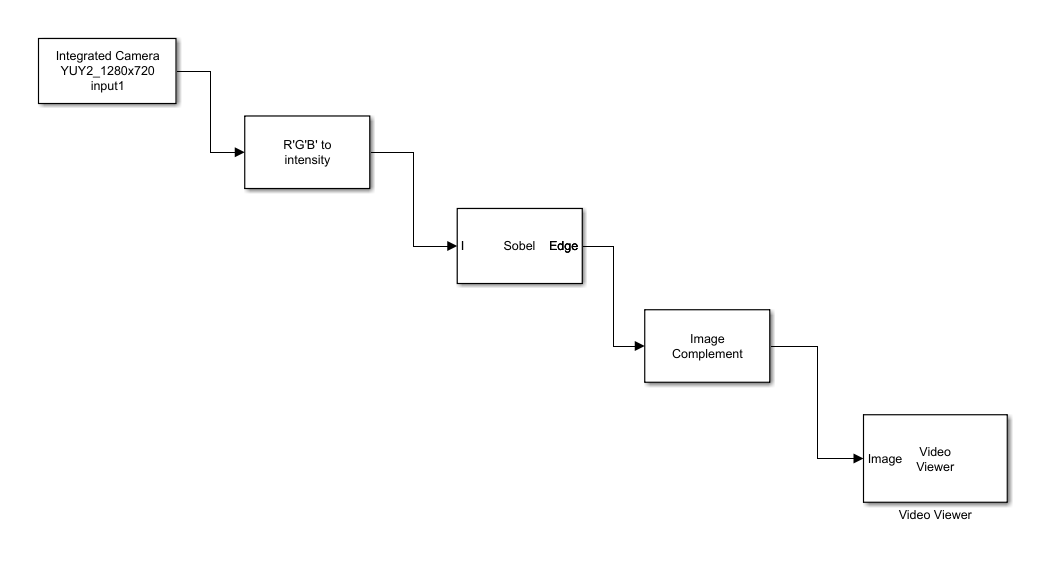
\includegraphics[width=15cm]{img.png}
	\end{figure*}
	
	\subsubsection{Ejecución}
	
	\begin{figure*}[!]
		\centering
		
\includegraphics[width=15cm]{img2.png}
	\end{figure*}
	
	\newpage
	
	\section{Conclusión}
	
	Este ejercicio nos ha brindado una experiencia práctica en el procesamiento de imágenes utilizando herramientas de simulación. Además, nos ha permitido comprender cómo los bloques en Simulink se pueden interconectar para crear flujos de trabajo complejos y realizar operaciones en tiempo real. Esta práctica sienta las bases para el desarrollo de soluciones más avanzadas en el campo del procesamiento de imágenes y nos abre las puertas a explorar nuevas técnicas y algoritmos en futuros proyectos.
	
\end{document}